\documentclass{article}
\usepackage{amssymb}
\usepackage{amsmath}
\usepackage{theoremref}
\usepackage{graphicx}
\usepackage{kotex}
\newtheorem{assumption}{Assumption}
\begin{document}
    \section{실험 모형}
    실험에서 세포 성장에 영향을 미칠 것으로 기대되는 요소인 영양소, 성장 인자 1, 성장 인자 2의 농도를 각각 $\alpha_1,\alpha_2,\alpha_3$으로 설정하고 최적의 요소 수준을 각각 $M_1,M_2,M_3$으로 설정한다. 세포 성장률을 아래 세 공식의 합으로 가정한다.
    \begin{align}
        &\beta_1(\alpha_1-M_1)^2+\epsilon_1\\
        &\left\{\begin{matrix}
            \alpha_1>l_1 & \beta_2(\alpha_2-M_2)^2+\epsilon_2 \\
            else & 0
        \end{matrix}\right.\\
        &\left\{\begin{matrix}
            \alpha_1>l_2 & \beta_3(\alpha_3-M_3)^2+\epsilon_3 \\
            else & 0
        \end{matrix}\right.
    \end{align} 
    \begin{assumption}
        성장인자로 인한 세포 성장 촉진은 영양소가 최소 수준 $l$ 이상일 때 효과가 나타난다.
    \end{assumption}
    \begin{assumption}
        요인에 따른 세포 성장 촉진은 최적 요소 수준이 최댓값인 이차곡선의 형태로 나타난다.
    \end{assumption}
    세가지 식의 효과를 종합하면 다음과 같이 나타낼 수 있다. 
    \begin{align}
        \beta_1\alpha_1^2+\beta_2\alpha_2^2+\beta_3\alpha_3^2+\beta_4\alpha_1+\beta_5\alpha_2+\beta_6\alpha_3+\beta_7\alpha_1\alpha_2+\beta_8\alpha_1\alpha_3+\beta_9\alpha_2\alpha_3+\epsilon
    \end{align}
    \begin{assumption}
        조류 추출물에 존재하는 단백질 등이 성장인자의 조효소로 작용한다 하더라도 세포에 충분한 영양분을 공급하는 $l$ 농도 이상에서는 충분히 존재하기 때문에 성장인자에 의한 세포 성장 수준에는 영향을 주지 않는다. 
    \end{assumption}
    \begin{assumption}
        성장인자가 세포 성장 영향을 주는 경로가 어떻게 독립적인지 
    \end{assumption}
    \begin{assumption}
        농도 $l$ 이상에서 영양소에 의한 세포 성장 촉진효과는 최고값 X에서 일정 범위 내 값으로 표현 할 수 있다. 
    \end{assumption}
    위 가정에 따라 (4)를 다음과 같이 간단히 한다.
    \begin{align}
        \left\{\begin{matrix}
            \alpha_1>\mathbf{MAX}(l_1,l_2) & \beta_2\alpha_2^2+\beta_3\alpha_3^2+\beta_5\alpha_2+\beta_6\alpha_3+\beta_9\alpha_2\alpha_3+\epsilon_l \\ & \epsilon_l = \in \mathbf{NID}(E,\sigma^2)\\
            else & \beta_1\alpha_1^2+\beta_4\alpha_1+\epsilon
        \end{matrix}\right.
    \end{align}
    위 식 (5)에 따라 python으로 시뮬레이션을 진행하였다. \\
    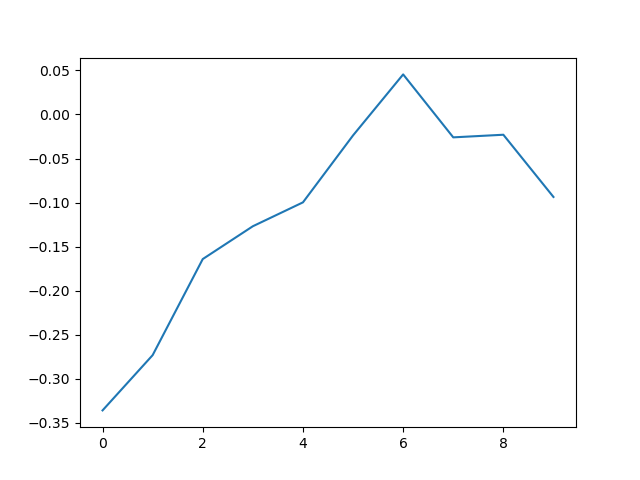
\includegraphics{Figure1.png} \\ 영양소 농도에 따른 세포 성장률 \\
    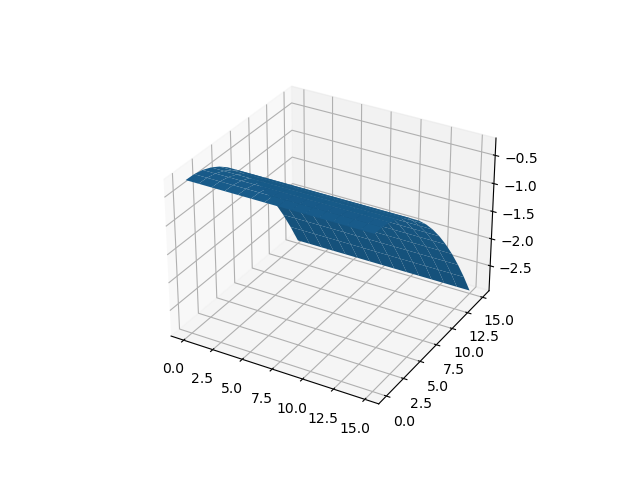
\includegraphics{Figure2.png} \\ 성장인자 농도에 따른 세포 성장률
\end{document}